%%%%%%%%%%%%%%%%%%%%%%%%%%%%%%%%%%%%%%%%%%%%%%%%%%%%%%%%%%%%%%%%%%%%%%
% main.tex
% Template de documento LaTeX para proyecto de fin de curso de Sistemas Embebidos para Tiempo Real
%
% Version 1.0 (IIE-FING-UDELAR)
% * Version inicial
%
%-- Leonardo Barboni, Julián Oreggioni
%    lbarboni@fing.edu.uy, juliano@fing.edu.uy
%
%%%%%%%%%%%%%%%%%%%%%%%%%%%%%%%%%%%%%%%%%%%%%%%%%%%%%%%%%%%%%%%%%%%%%%

\documentclass[a4paper,12pt]{article}

\usepackage{amsmath,amssymb}             
\usepackage{amsfonts}
\usepackage[utf8]{inputenc}   
\usepackage[spanish]{babel}
\selectlanguage{spanish} 
\usepackage[ruled,vlined,spanish]{algorithm2e}
\usepackage[T1]{fontenc}
\usepackage[left=2cm,right=2cm,top=1cm,bottom=1.5cm,includefoot,includehead,headheight=13.6pt]{geometry}
\usepackage{aecompl}
\usepackage[pdftex]{graphicx}
\graphicspath{{./figs/}}
\usepackage{color}
\usepackage{url}
\usepackage[font=small,labelfont=bf,tableposition=top]{caption}
\usepackage[most]{tcolorbox}
\usepackage{lineno}
\usepackage[numbers,sort&compress]{natbib}
\usepackage{listings}
\usepackage{fancyhdr, lastpage}
\usepackage{longtable}
\usepackage{afterpage}
\usepackage{textcomp}

\hyphenpenalty=13000

%----------------------                      
\pagestyle{fancy} 
\fancyhf{}                                             
\fancyfoot[C]{\hrule \bfseries\thepage}                   
\fancyhead[C]{\bfseries\nouppercase{Proyecto - Sistemas Embebidos Para Tiempo Real - 2020}}     

\fancypagestyle{firstpage}{
\pagestyle{fancy} 
\fancyhf{}                                             
\fancyfoot[C]{\hrule}                   
\fancyhead[C]{\bfseries\nouppercase{Proyecto - Sistemas Embebidos Para Tiempo Real - 2020}}     
}

%+++++++++++++++

\renewcommand{\contentsname}{Tabla de Contenido}
\renewcommand{\listtablename}{Índice de tablas}
\renewcommand{\tablename}{Tabla} 

%+++++++++++++++

\begin{document} 

\thispagestyle{firstpage}

\begin{linenumbers} %COMENTAR PARA SACAR NUMERACION DE LINEAS

\tcbset{
    frame code={},
    center title,
    left=0pt,
    right=0pt,
    top=0pt,
    bottom=0pt,
    colback=gray!70,
    colframe=white,
    width=\dimexpr\textwidth\relax,
    enlarge left by=0mm,
    boxsep=5pt,
    arc=0pt,outer arc=0pt,
    }



\vspace{0.5in}
\begin{tcolorbox}
\vspace{2pc}
\centerline{\sc \large \textbf {Titulo del Proyecto}}
\vspace{1pc}
\centerline{\sc \large \textbf {Nombre corto del proyecto}}
\vspace{1pc}
\centerline{\sc \textbf {Autores:} Autor 1, Autor 2, Autor 3 }
\vspace{2pc}
\centerline{\textbf {Emails:} estudiante1@fing.edu.uy, estudiante2@fing.edu.uy, estudiante3@fing.edu.uy}
\vspace{2pc}
\end{tcolorbox}
\centerline{\textbf {Tutores}: Tutor 1 y Tutor 2}
\vspace{1pc}
\centerline{\textbf {Emails:} tutor1@fing.edu.uy, tutor2@fing.edu.uy}
\vspace{2pc}
\centerline{Instituto de Ingenier\'ia El\'ectrica - Facultad de Ingenier\'ia - UDELAR}
\vspace{2pc} 
\noindent\rule{17cm}{0.4pt}
\vspace{2pc}



\tcbset{
    frame code={}
    center title,
    left=0pt,
    right=0pt,
    top=0pt,
    bottom=0pt,
    colback=gray!20,
    colframe=white,
    width=\dimexpr\textwidth\relax,
    enlarge left by=0mm,
    boxsep=5pt,
    arc=0pt,outer arc=0pt,
    }

\begin{tcolorbox}
\textsc{\textbf{Resumen}}\\
\newline
Resumir el proyecto en no mas de 200 palabras. Recordar que la documentaci\'on no debe superar las 25 carillas, sin incluir esta car\'atula ni la 
tabla de contenidos o anexos. Recuerde que el resumen es una descripci\'on corta, concreta y clara de los temas desarrollados, as\'i como tambi\'en de los m\'etodos y herramientas utilizados y de los resultados obtenidos. Agregar una muy breve descripci\'on de las conclusiones a las que se ha llegado.
\end{tcolorbox}

%+++++++++++++++++++++++

\newpage
\setcounter{page}{1}
\tableofcontents

%+++++++++++++++++++++++
\section{Introducci\'on}
\label{sec:introduccion}

Este es un template para la documentaci\'on del proyecto de fin del curso Sistemas Embebidos para Tiempo Real (SiSem) y en 2020 fue la primera vez que se puso en pr\'actica. Por esto, en la documentaci\'on de proyectos de ediciones anteriores de SiSem presentan una gran diversidad de formatos. De cualquier manera, recomendamos revisar la documentaci\'on de proyectos de a\~nos anteriores disponibles en la p\'agina del curso.

La introducción se puede ilustrar con alguna figura (ver Fig.~\ref{fig:autos}). Tener presente que todas las figuras deben estar referenciadas en el texto. Las figuras deben estar en formato pdf (deben ser generadas en formato vectorizado .eps, .ps, o .svg y luego convertidas a .pdf para incorporar al documento). En la fuente latex de este documento se puede mirar cómo insertar una figura, como la Fig.~\ref{fig:autos}. Las referencias deben estar citadas por orden de aparici\'on (por ejemplo as\'i~\cite{arbio2015}\cite{CodeComposer}\cite{Alley2018}\cite{Olloniego2019}\cite{Dang2015}\cite{Branco2019}) y en formato IEEE con un archivo bibtex. Con este template se adjunta un archivo bibtex de ejemplo (ver \textit{refs.bib}) y el archivo \textit{IEEEtran\_bst\_HOWTO.pdf} que explica en detalle cómo armar las referencias.

La numeraci\'on de l\'ineas a la izquierda (l\'inea a l\'inea) deben dejarse para la entrega del documento borrador que los docentes van a corregir, pero para la entrega final que se va a subir a EVA deben quitarse. Para eso deben comentarse las líneas que dicen \verb!\begin{linenumbers}! y~\verb!\end{linenumbers}!.

%-----------------
\begin{figure}[ht]
  \begin{center}
    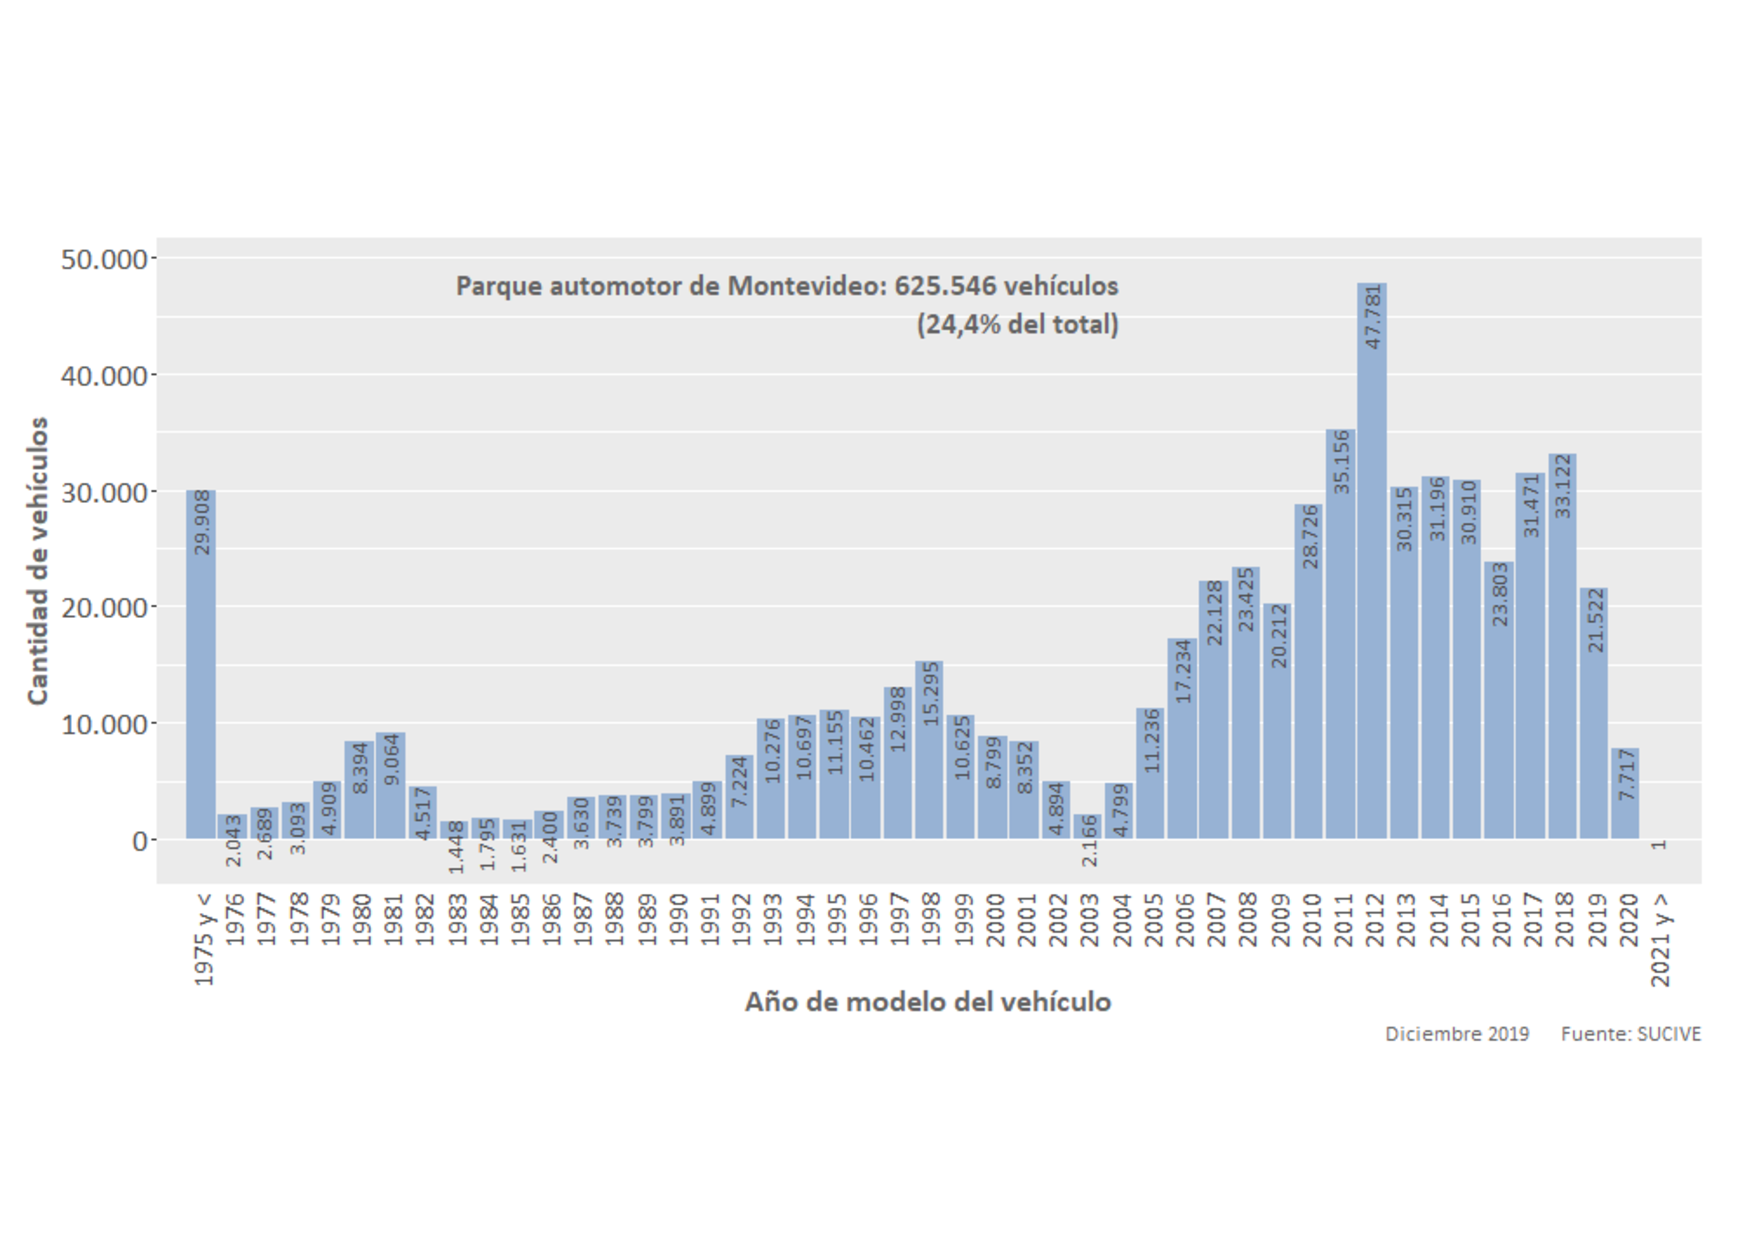
\includegraphics[width=1\textwidth]{autos.pdf}
  \end{center}
  \caption{Evolución del parque automotor de Montevideo (reproducida de~\cite{mtop2020}). \textit{Todas las figuras deben estar referenciadas y explicadas en el texto y adem\'as indicar de dónde fueron copiadas si no son originales, por ejemplo decir: figura adaptada o reproducida de~[X].}}
  \label{fig:autos}
\end{figure}
%-----------------


\subsection{Descripci\'on del problema}
\label{sec:problema}

Describir el problema que será abordado. No solo se debe explicar brevemente el problema a nivel de aplicaci\'on sino que deben quedar identificados claramente los sub-problemas de sistemas embebidos que se tuvieron que resolver. 

\subsection{Antecedentes} 
\label{sec:antencedentes}

Mencionar brevemente proyectos anteriores, art\'iculos, libros, soluciones disponibles, etc., y cómo se relacionan con este proyecto.  

%++++++++++++++++++
\section{Objetivos}
\label{sec:objetivos}

Indicar brevemente los objetivos del proyecto planteados en la especificación detallada. Se pide los objetivos relacionados al curso y no otros. Pueden dividirse entre un objetivo general, y algunos objetivos específicos.

%++++++++++++++++++
\section{Alcance}
\label{sec:alcance}

Definir el alcance del proyecto, establecer qu\'e parte del problema presentado en la Sección \ref{sec:problema} se va resolver en el marco del presente proyecto. Decir qué se incluye dentro del proyecto y también qu\'e no. 

Si el problema que se está abordando está asociado a un proyecto de fin de carrera, especificar  el alcance de ambos, diferenciando qué es lo que entra en el \'area de SiSem. 


%++++++++++++++++++++++++++++++++++
\section{Descripci\'on del Sistema}
\label{sec:sistema}

Esta sección debe contener la descripción de la solución que este trabajo propone para el problema propuesto en la Sección \ref{sec:problema}. La solución se nutre de los trabajos previos mencionados en la Sección \ref{sec:antencedentes}, y pretende resolver el problema total o parcialmente de acuerdo a los objetivos y alcance definidos en las Secciones \ref{sec:objetivos} y \ref{sec:alcance}.

Se debe realizar una descripción funcional de la implementaci\'on (responder a las preguntas ¿Qué hace el sistema? ¿Cómo funciona?). La descripción deberá realizarse en texto con fuerte apoyo de diagramas de alto nivel (ver Figs. \ref{fig:vacas} y \ref{fig:guri}). Se trata de la descripci\'on general del sistema y no se debe entrar en la descripci\'on interna de los bloques de hardware ni de software (esto se realiza en la Secci\'on \ref{sec:implementacion}). Asimismo, deberá agregarse toda otra informaci\'on de carácter general que se considere relevante para describir el funcionamiento del sistema. Por ejemplo, si se considera necesario se podrán incluir diagramas de tiempos (pero siempre desde una perspectiva global).


\begin{figure}[ht]
  \begin{center}
    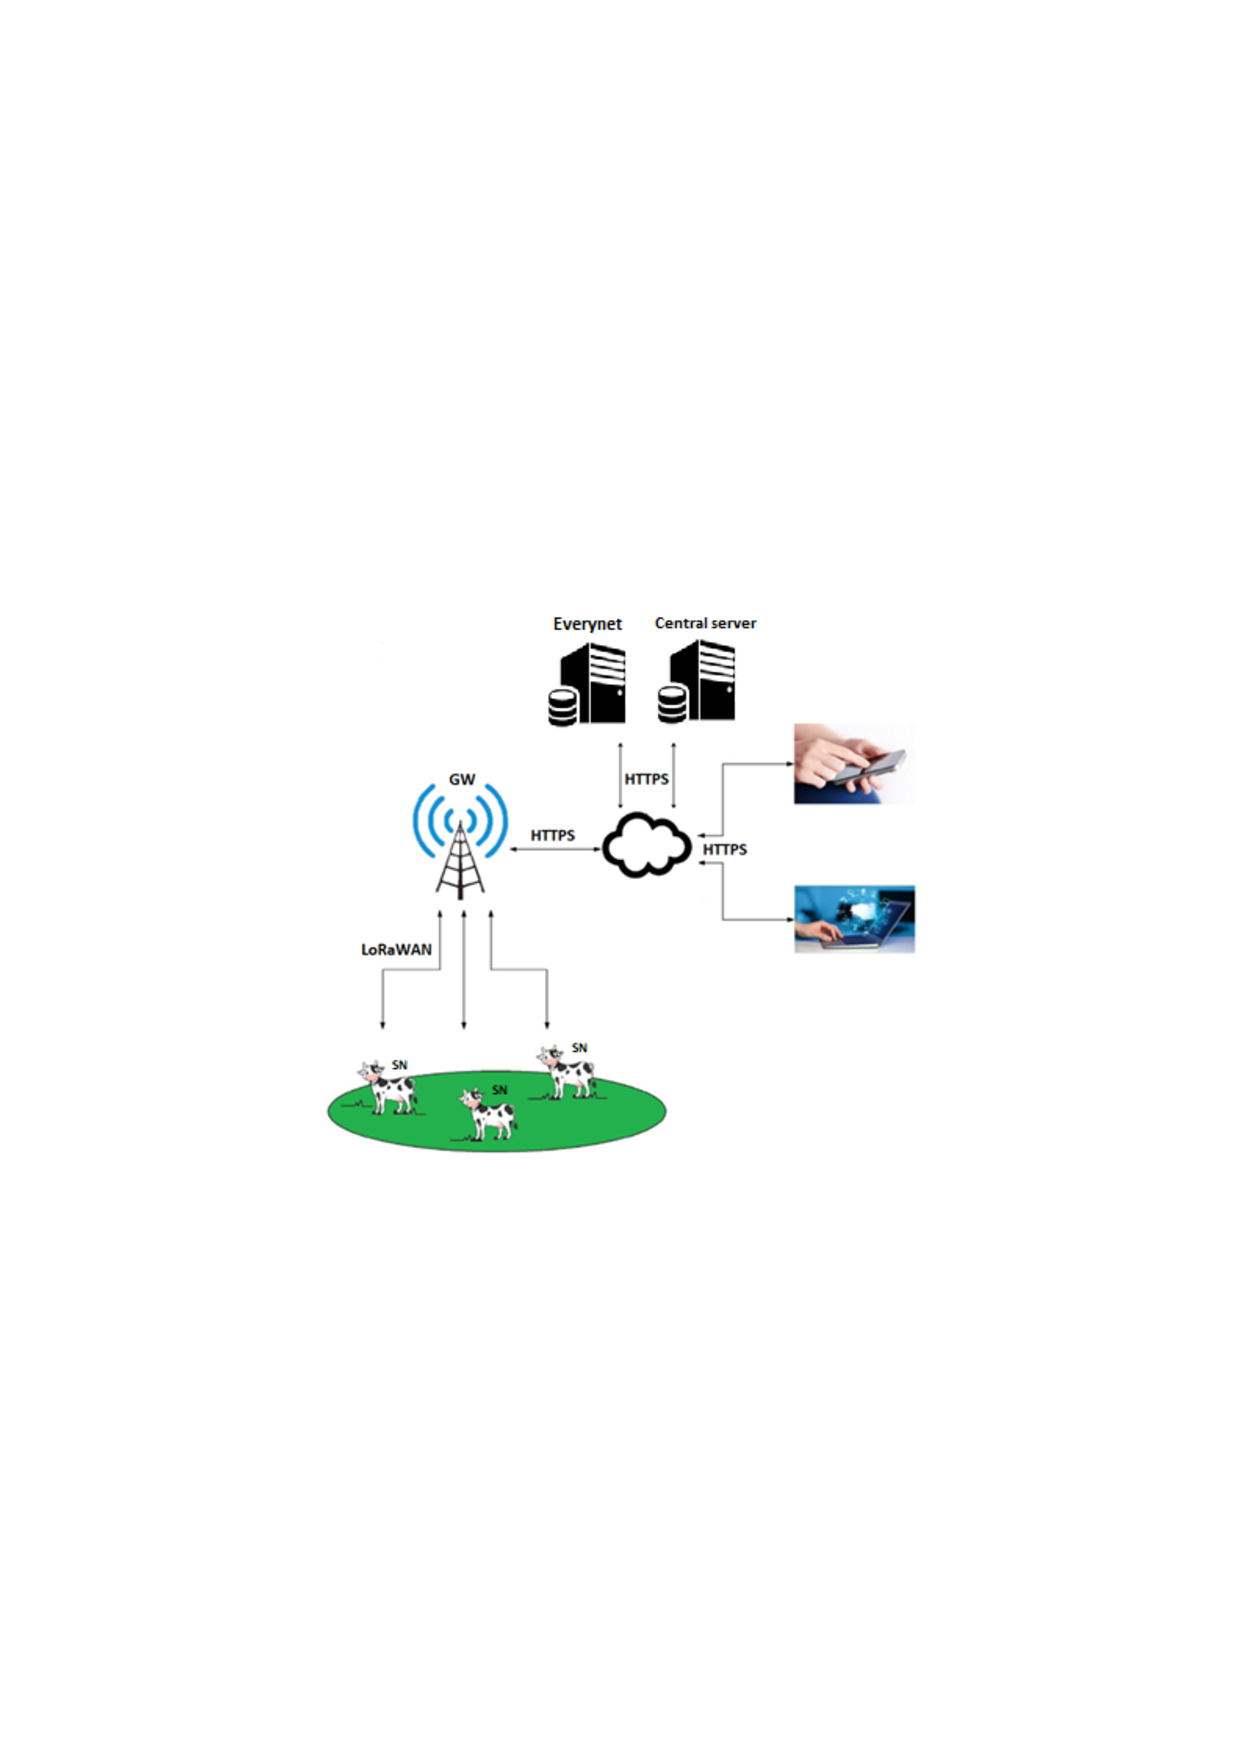
\includegraphics[width=0.6\textwidth]{vacas.pdf}
  \end{center}
  \caption{Diagrama funcional de alto nivel, reproducida de~\cite{acosta2020}. }
  \label{fig:vacas}
\end{figure}

\begin{figure}[ht]
  \begin{center}
    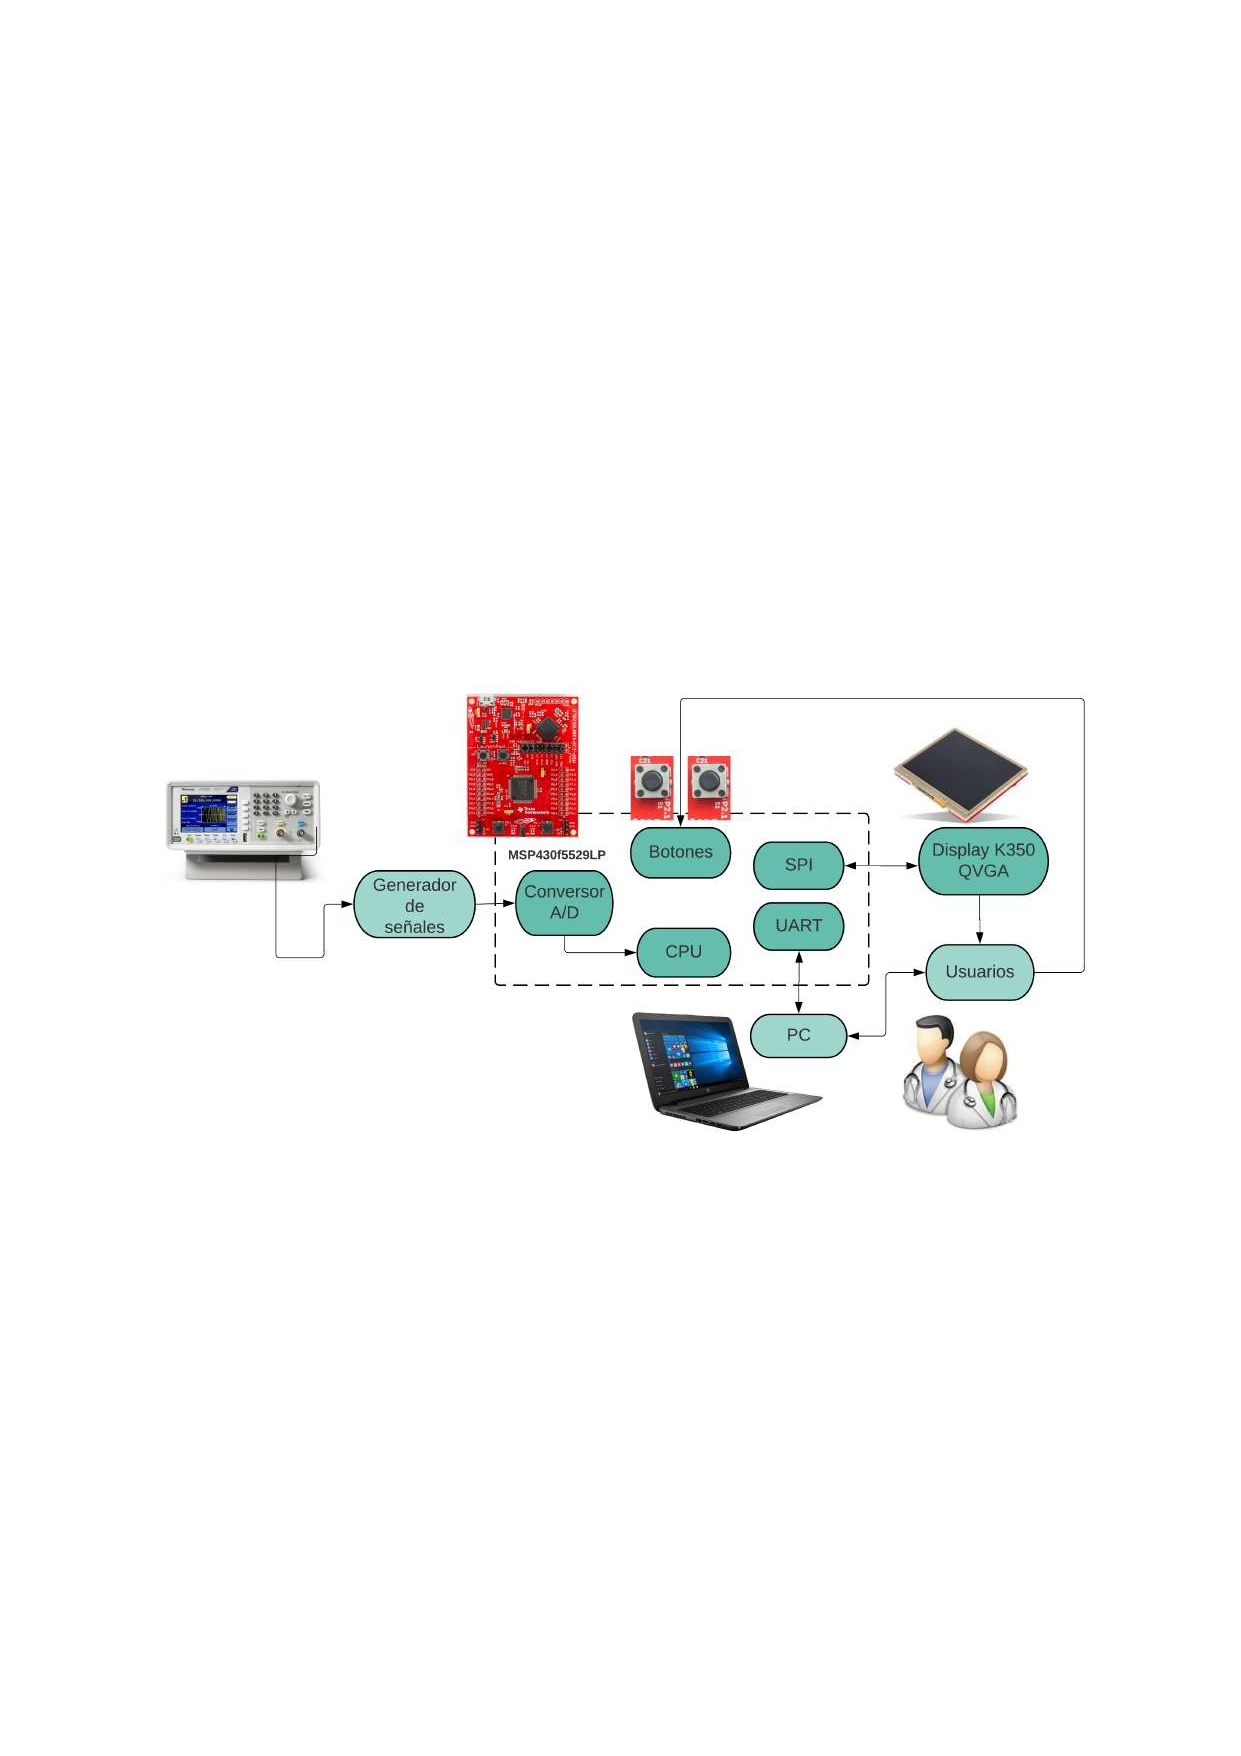
\includegraphics[width=0.7\textwidth]{guri.pdf}
  \end{center}
  \caption{Diagrama funcional con cierto detalle a nivel de bloques, reproducida de~\cite{cabrera2019}. }
  \label{fig:guri}
\end{figure}



%++++++++++++++++++++++++++++++++++
\section{Implementac\'ion}
\label{sec:implementacion}

Esta secci\'on se divide en dos partes y será el n\'ucleo de la documentaci\'on. Debe incluir información del tool-chain y/o IDE usado.

%++++++++++++++++++++++++++++++++++
\subsection{Hardware}
\label{sec:hardware}

En esta secci\'on se describe el hardware utilizado, en particular aclarar y detallar si se tuvo que desarrollar hardware específico. Utilizar diagramas con los bloques constitutivos señalando cómo comunican entre ellos (Diagrama de Bloques) y/o Diagramas funcionales (Ver Figs. \ref{fig:guri} y  \ref{fig:dhbewsdc}). Si corresponde, poner referencias a Notas de Aplicación o cualquier material utilizado. Poner diagramas esquem\'aticos de los circuitos y diagrama de conexi\'on de bloques con pin-out (dependiendo del tamaño y complejidad pueden colocarse en un anexo). Para cada bloque constitutivo de hardware, as\'i sea parte del interior del microcontrolador o no, debe indicarse que toma como entrada, de donde, y con qué otros bloques está interconectado. Indicar en el diagrama los buses y pines I/O usados, tensi\'ones de alimentaci\'on, etc.

%-----------------
\begin{figure}[ht]
  \begin{center}
    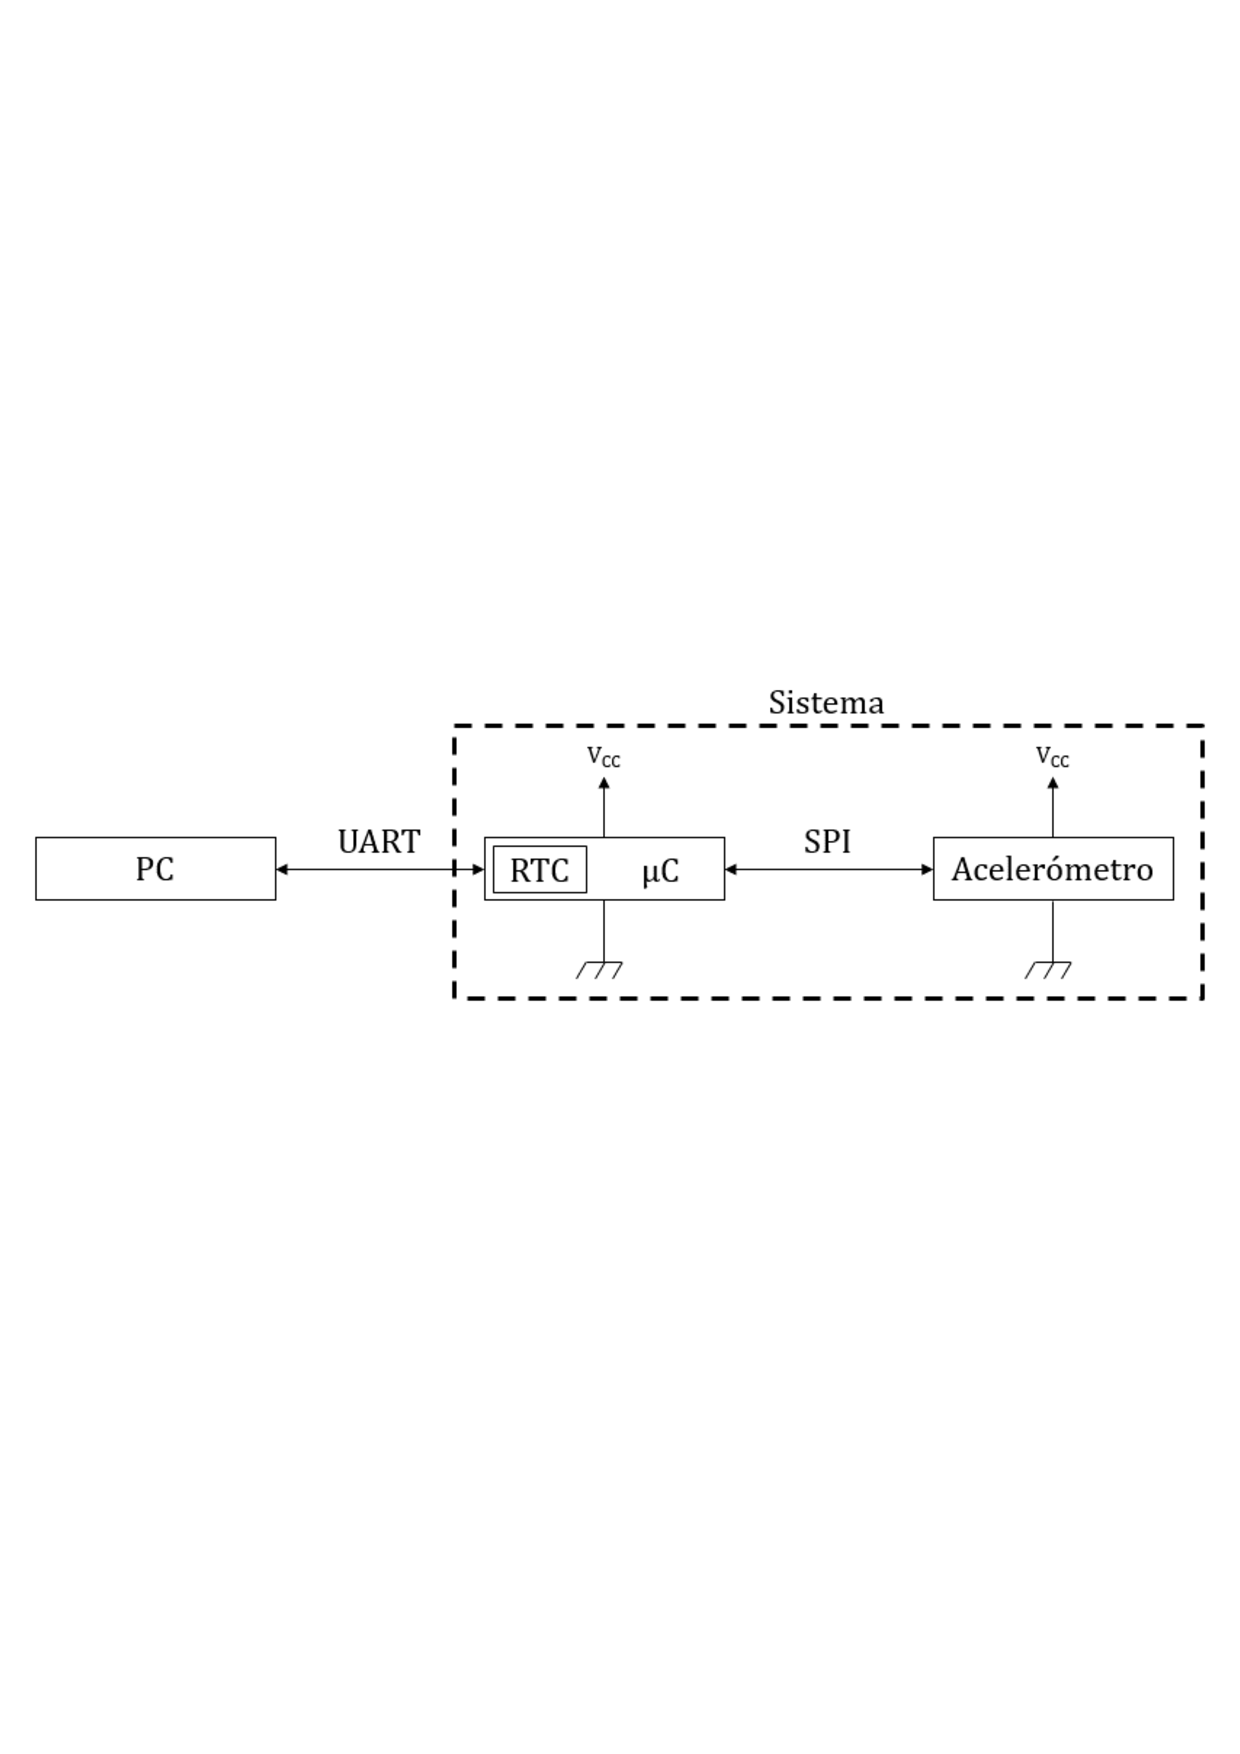
\includegraphics[width=0.7\textwidth]{bloques.pdf}
  \end{center}
  \caption{Diagrama de bloques (reproducida de \cite{facal2017}). }
  \label{fig:dhbewsdc}
\end{figure}
%-----------------

%++++++++++++++++++++++++++++++++++
\subsection{Software}
\label{sec:software}


Se deben adjuntar diagrama de módulos con división jer\'arquica (Diagrama de Módulos). Ver Fig. \ref{fig:insulogger}. Para cada capa, o m\'odulo, o funci\'on se debe indicar qué variables tiene como entradas, de qui\'en recibe dichas entradas, qué variables internas utiliza (y en qué formato, y el encapsulamiento, o sea qué variables son accesibles y cuáles privadas). Se debe indicar adem\'as qué funciones cumplen dentro de la implementaci\'on y con qué otro bloque,  m\'odulo o funci\'on se comunica  para proporcionar resultados, comandos, informaci\'on o manejar perif\'ericos (se sugiere agregar las dependencias en los diagramas). 

%-----------------
\begin{figure}[ht]
  \begin{center}
    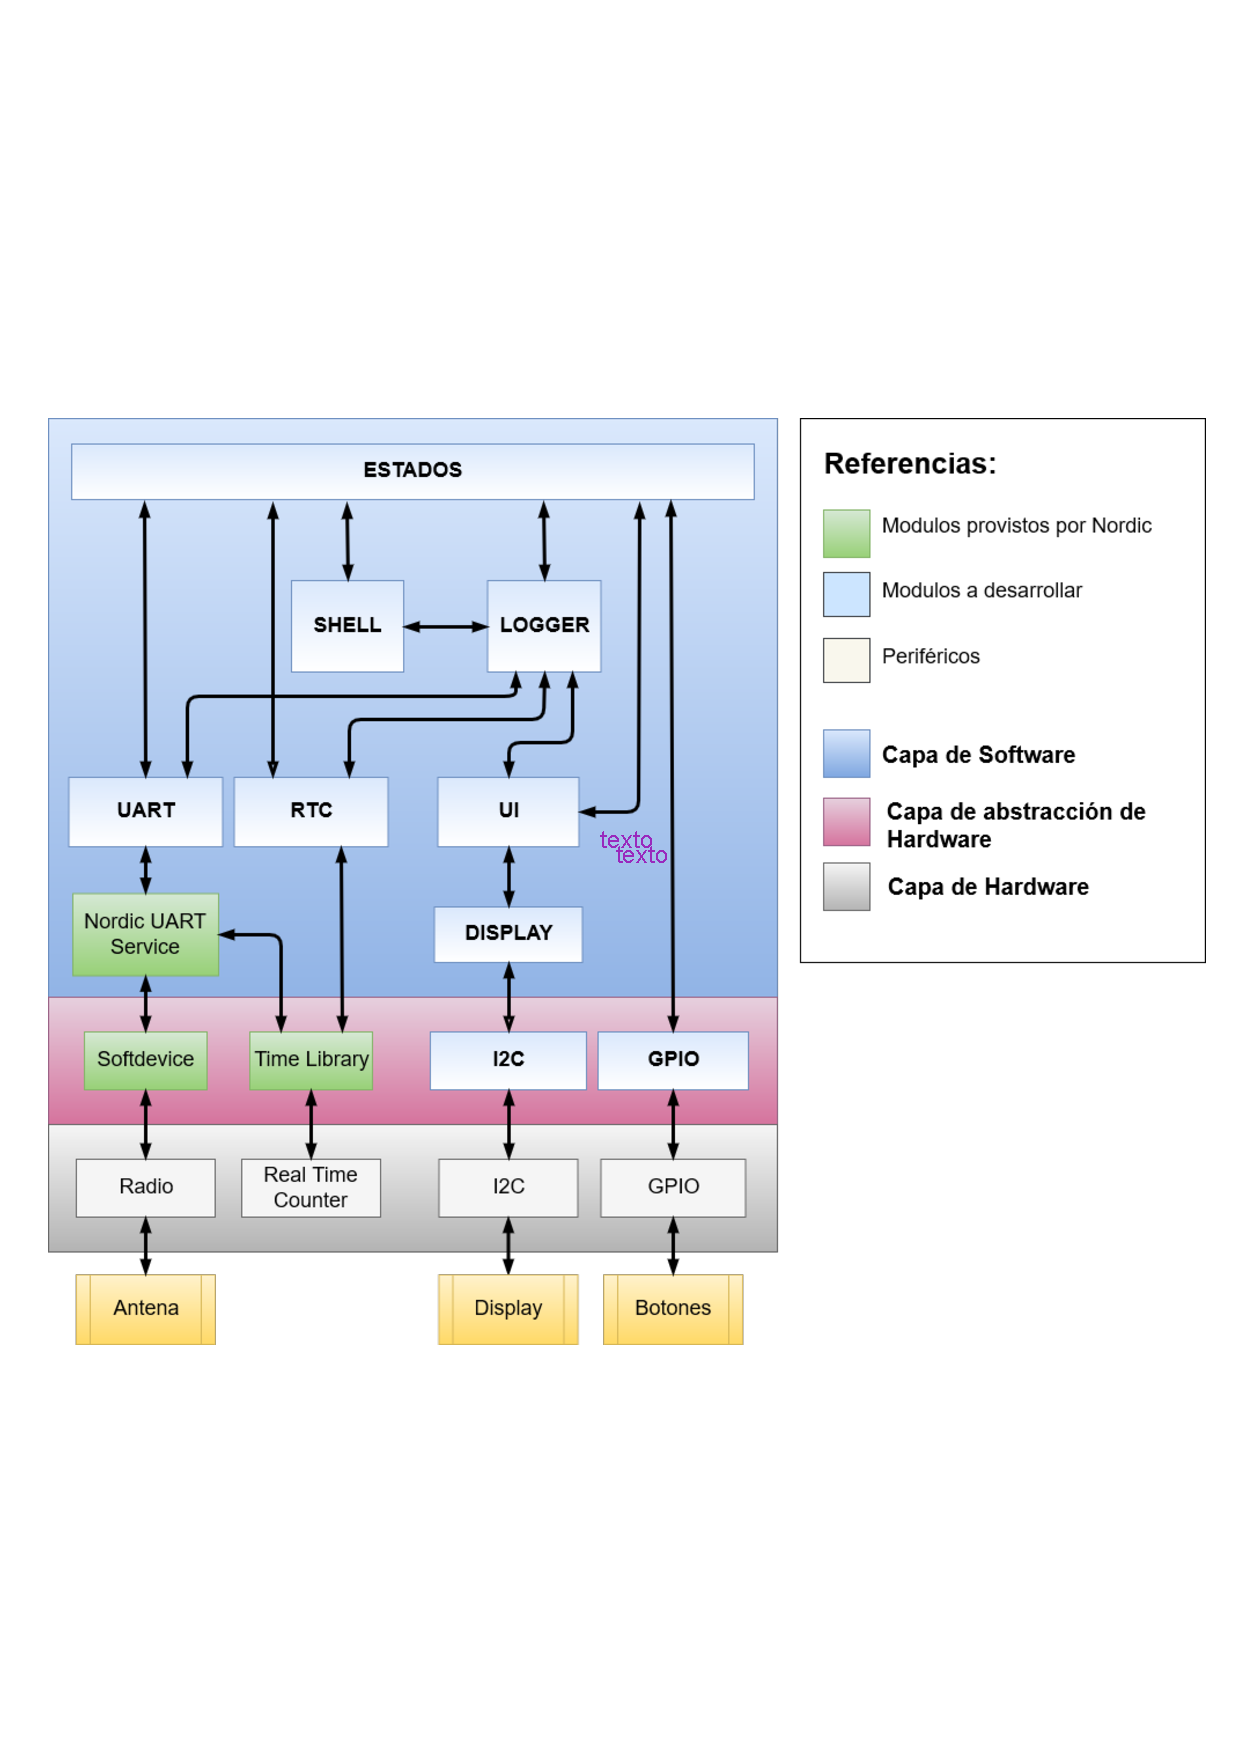
\includegraphics[width=\textwidth]{insulogger.pdf}
  \end{center}
  \caption{Diagrama de módulos. Se muestra la jerarqu\'ia, separando entre hardware y software (reproducida de \cite{Bentancour2018}). }
  \label{fig:insulogger}
\end{figure}
%-----------------

Se sugiere poner pseudocodigo de las partes que se consideren importantes del c\'odigo utilizando el formato presentando para los algoritmos \ref{algo:muestra} y \ref{algo:max}.

%===================
\begin{algorithm}[H]
\SetAlgoLined
\KwIn{entradas del algoritmo}
\KwOut{salidas del algoritmo}
\KwResult{resumir muy brevemente qué hace, a qué se corresponde esa salida (como función de las entradas)}
 Inicializaci\'on (variables locales, y si correponde variables globales)\;
 \While{{$Condition \geq 1$}}{
  instructions\;
  \eIf{condition $something \not= 0$}{
   instructions1\;
   instructions2\;
   Reviso flag, TX, entrar a LPM3, etc.\;
   $d = \min \{c,e\}$\tcp*[r]{puedo agregar comentario acá}
   }{
  $var1 \leftarrow var2$\;                          
  }
 }
 \caption{{\sc Ejemplo de cómo escribir pseudoc\'odigo:} esto es el nombre del algoritmo (puede ser una función, parte del main, una ISR o un algoritmo propiamente). }
  \label{algo:muestra}
\end{algorithm}
\vspace*{2pc}

\begin{algorithm}
\DontPrintSemicolon % puede ser necesarios usar \dontprintsemicolon 
\KwIn{Un conjunto finito de números enteros $A=\{a_1, a_2, \ldots, a_n\}$}
\KwOut{El entero mayor que pertenece al conjunto $A$}
$max \gets a_1$\;
\For{$i \gets 2$ \textbf{to} $n$} {
  \If{$a_i > max$} {
    $max \gets a_i$\;
  }
}
\Return{$max$}\;
\caption{{\sc Maximo:} encuentra el máximo}
\label{algo:max}
\end{algorithm}
%===================

También se puede documentar la implementación del software embebido mediante diagramas de flujo, ver en Figs.~\ref{fig:sdcs123432zbkof} y~\ref{fig:ijndse320jdnbw3rfa}. Incorporar diagramas de flujo del \textit{main} y las \textit{ISR}, diagramas de estados (ver Fig. \ref{fig:estados}), o de m\'aquinas de estados (ver Fig. \ref{fig:maquina}) si corresponde. 


%-----------------
\begin{figure}[ht]
  \begin{center}
    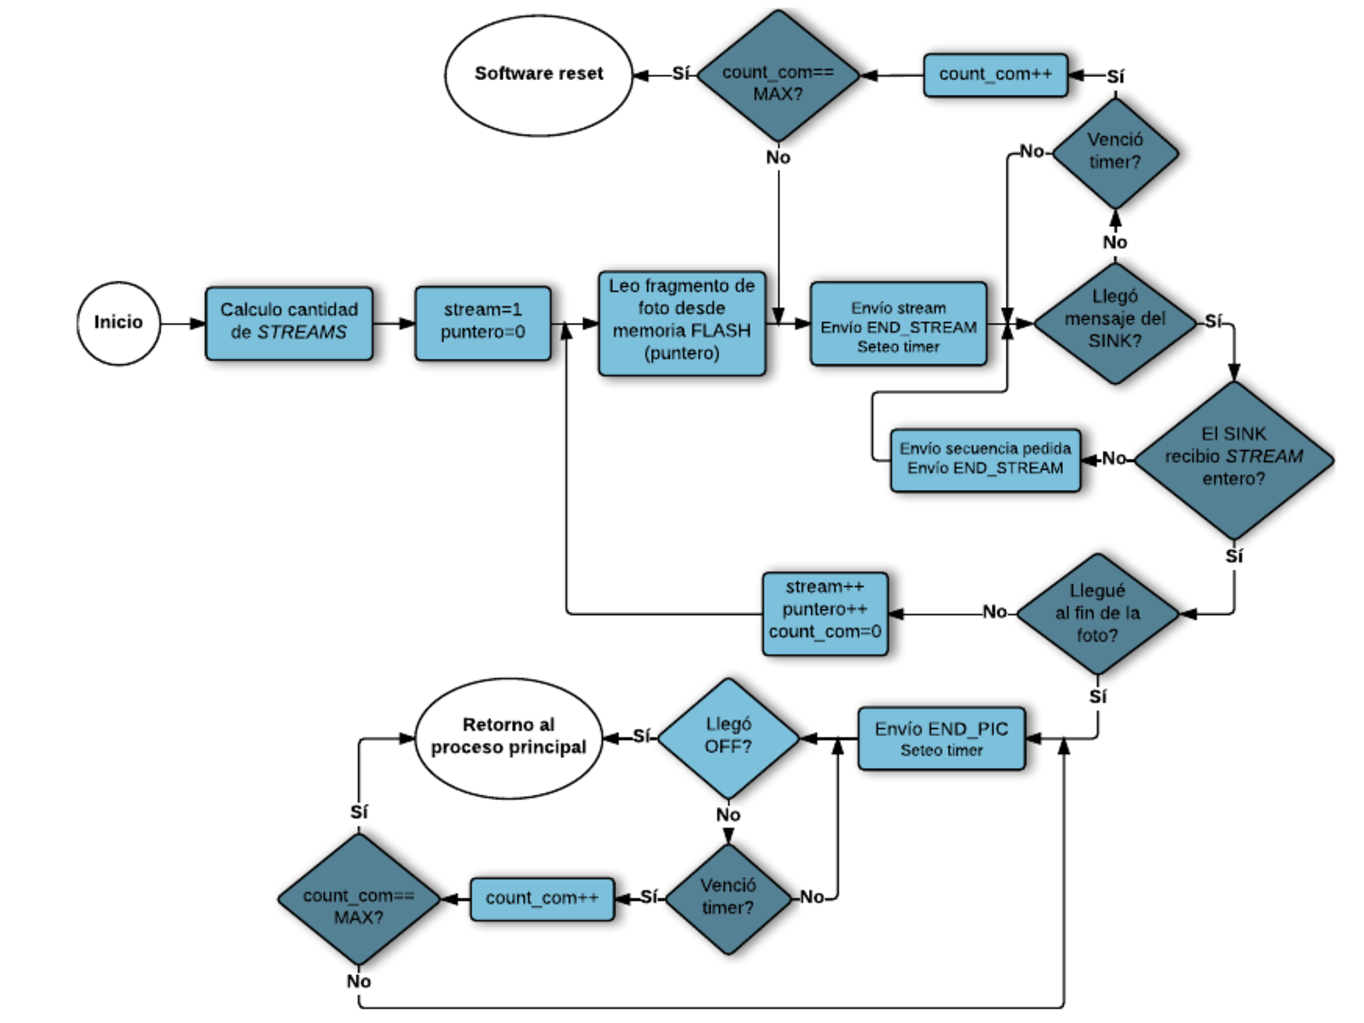
\includegraphics[width=0.9\textwidth]{figura4.pdf}
  \end{center}
  \caption{Diagrama de flujo de una función (reproducida de \cite{arbio2015}). }
  \label{fig:sdcs123432zbkof}
\end{figure}
%-----------------

%-----------------
\begin{figure}[ht]
  \begin{center}
    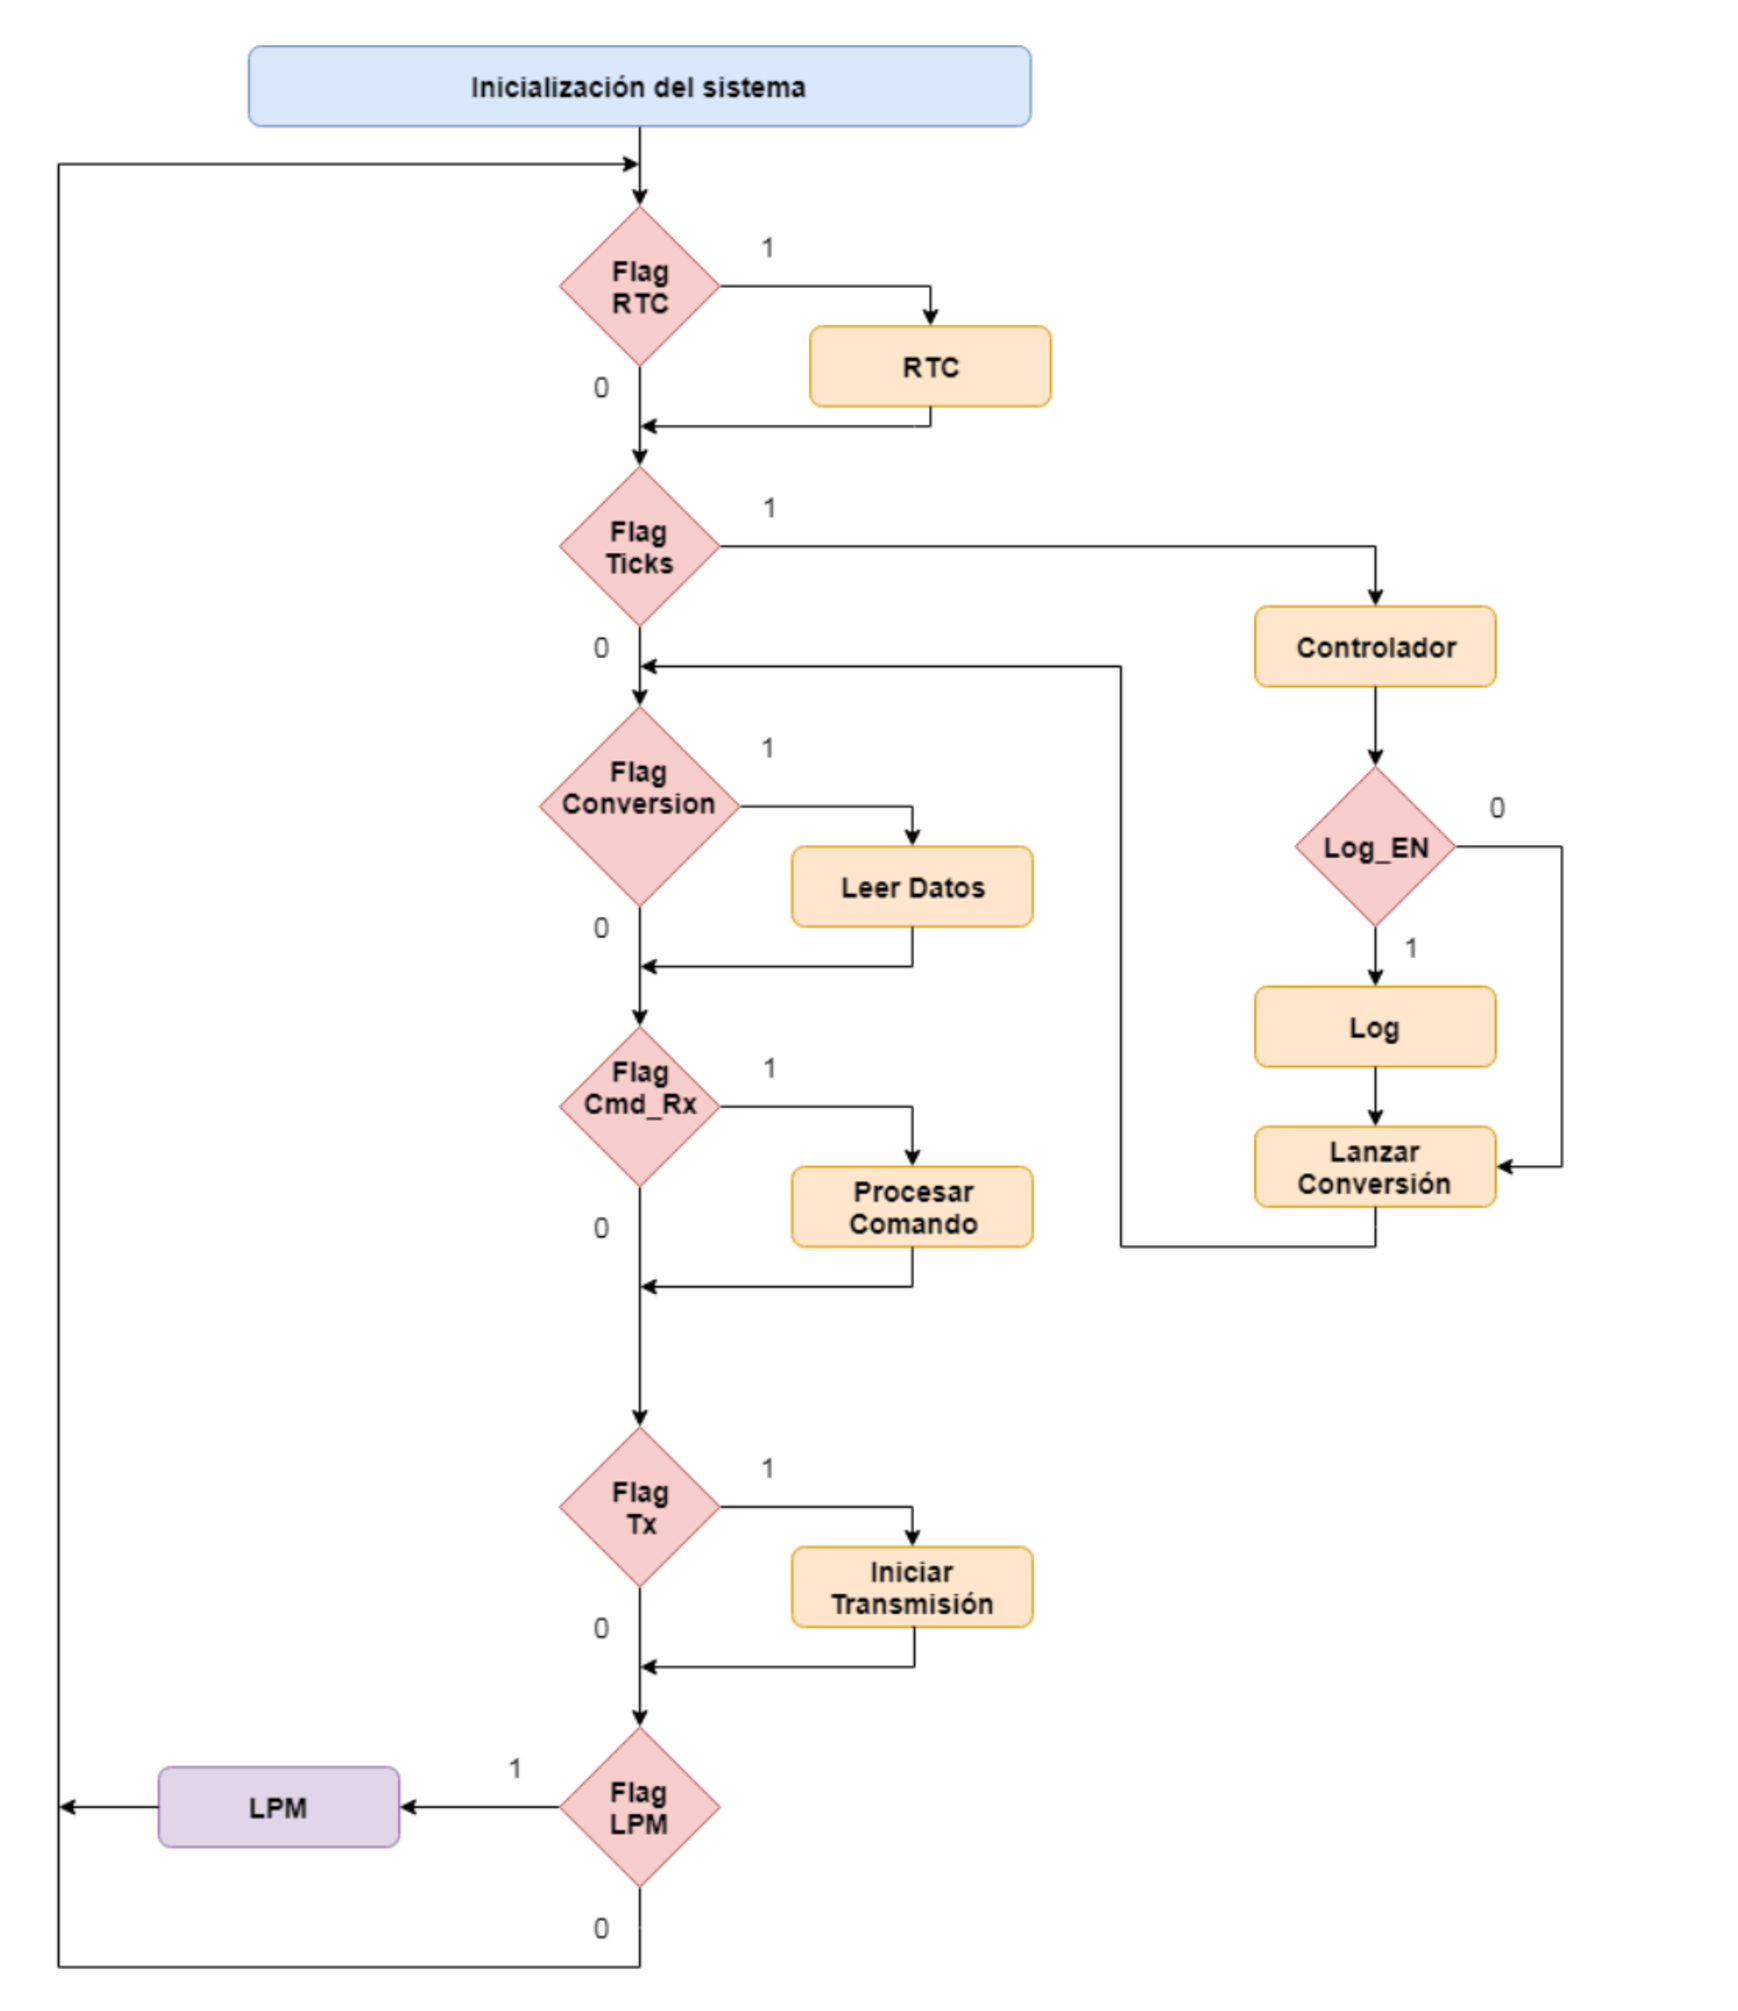
\includegraphics[width=0.75\textwidth]{figura5.pdf}
  \end{center}
  \caption{Diagrama de flujo del main, detalle del Round-Robin con interrupciones (reproducida de \cite{Iglesias2019}). }
  \label{fig:ijndse320jdnbw3rfa}
\end{figure}
%-----------------

%-----------------
\begin{figure}[ht]
  \begin{center}
    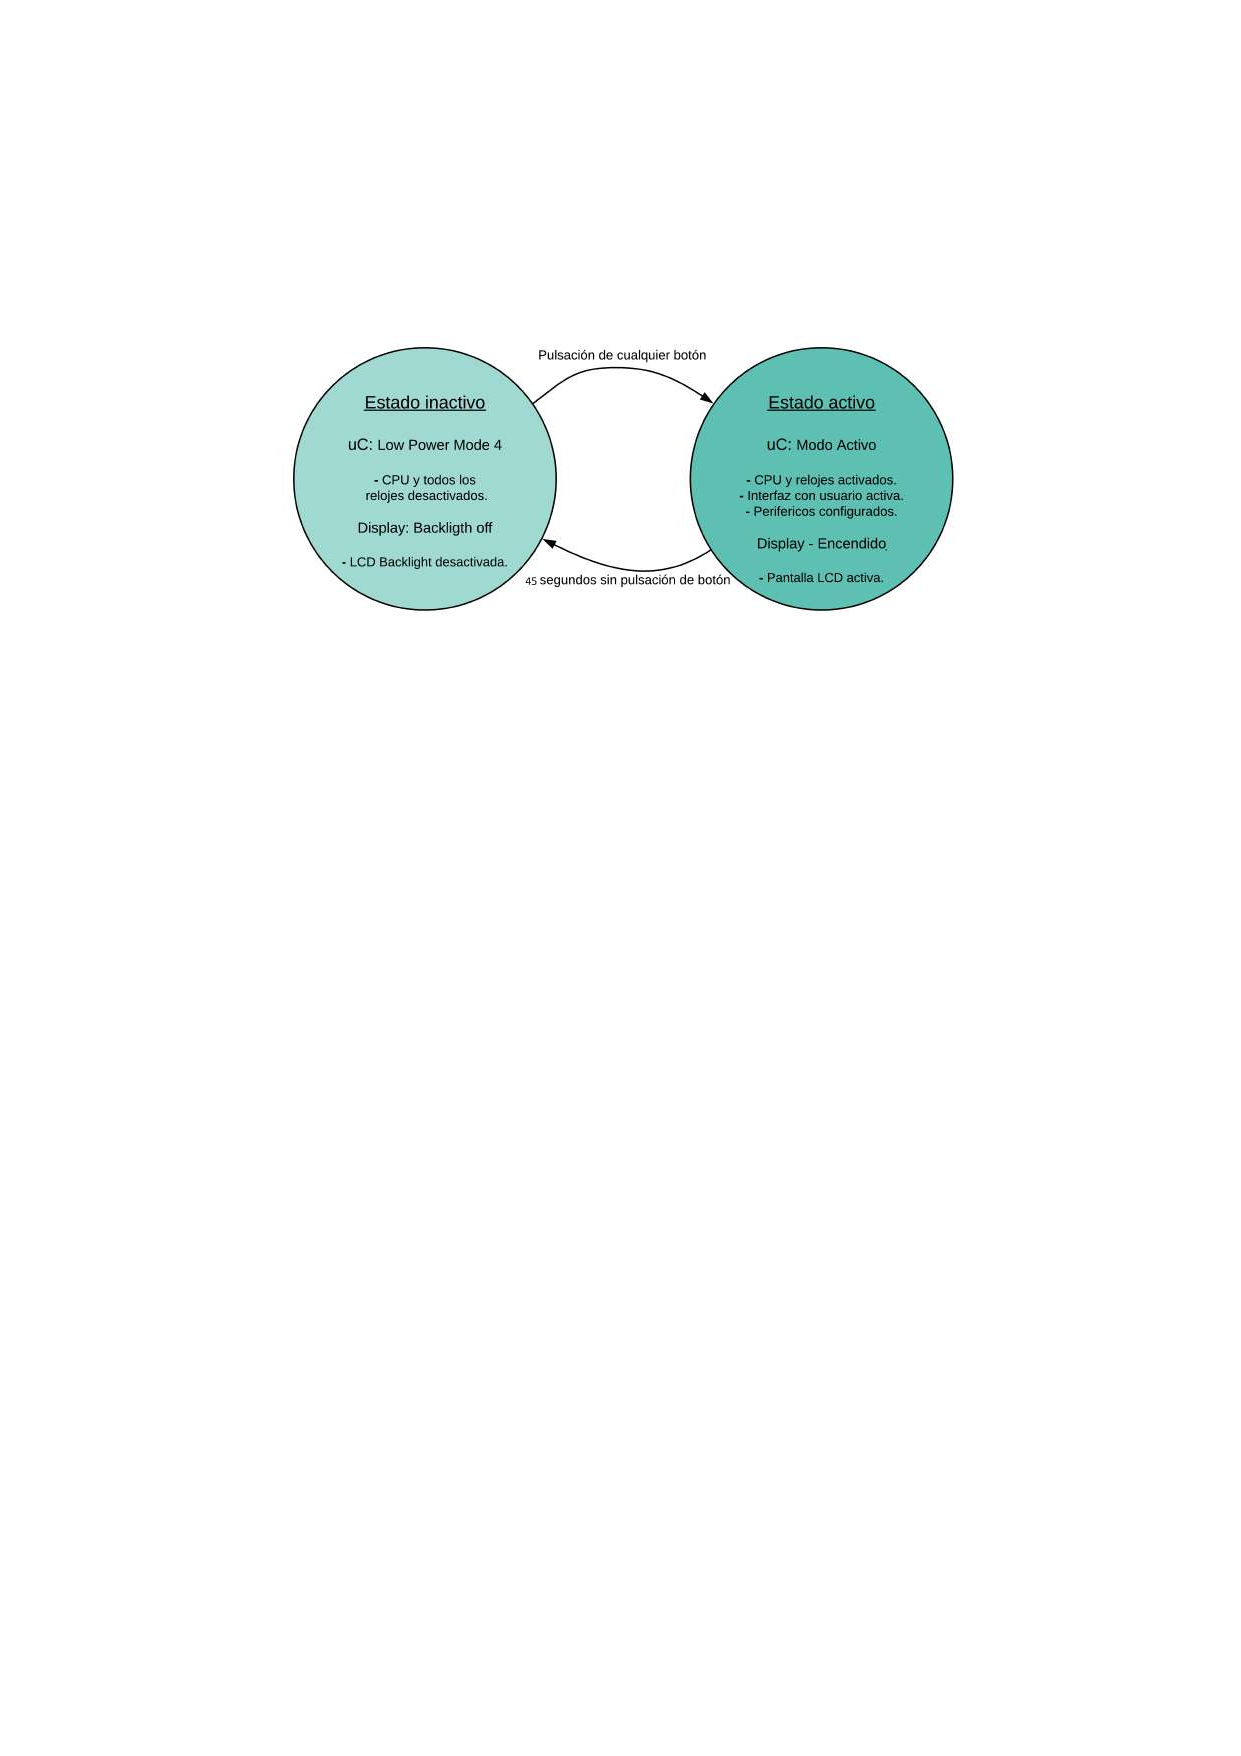
\includegraphics[width=0.6\textwidth]{estados.pdf}
  \end{center}
  \caption{Diagrama según estados del microcontrolador (reproducida de \cite{cabrera2019}). }
  \label{fig:estados}
\end{figure}
%-----------------

%-----------------
\begin{figure}[ht]
  \begin{center}
    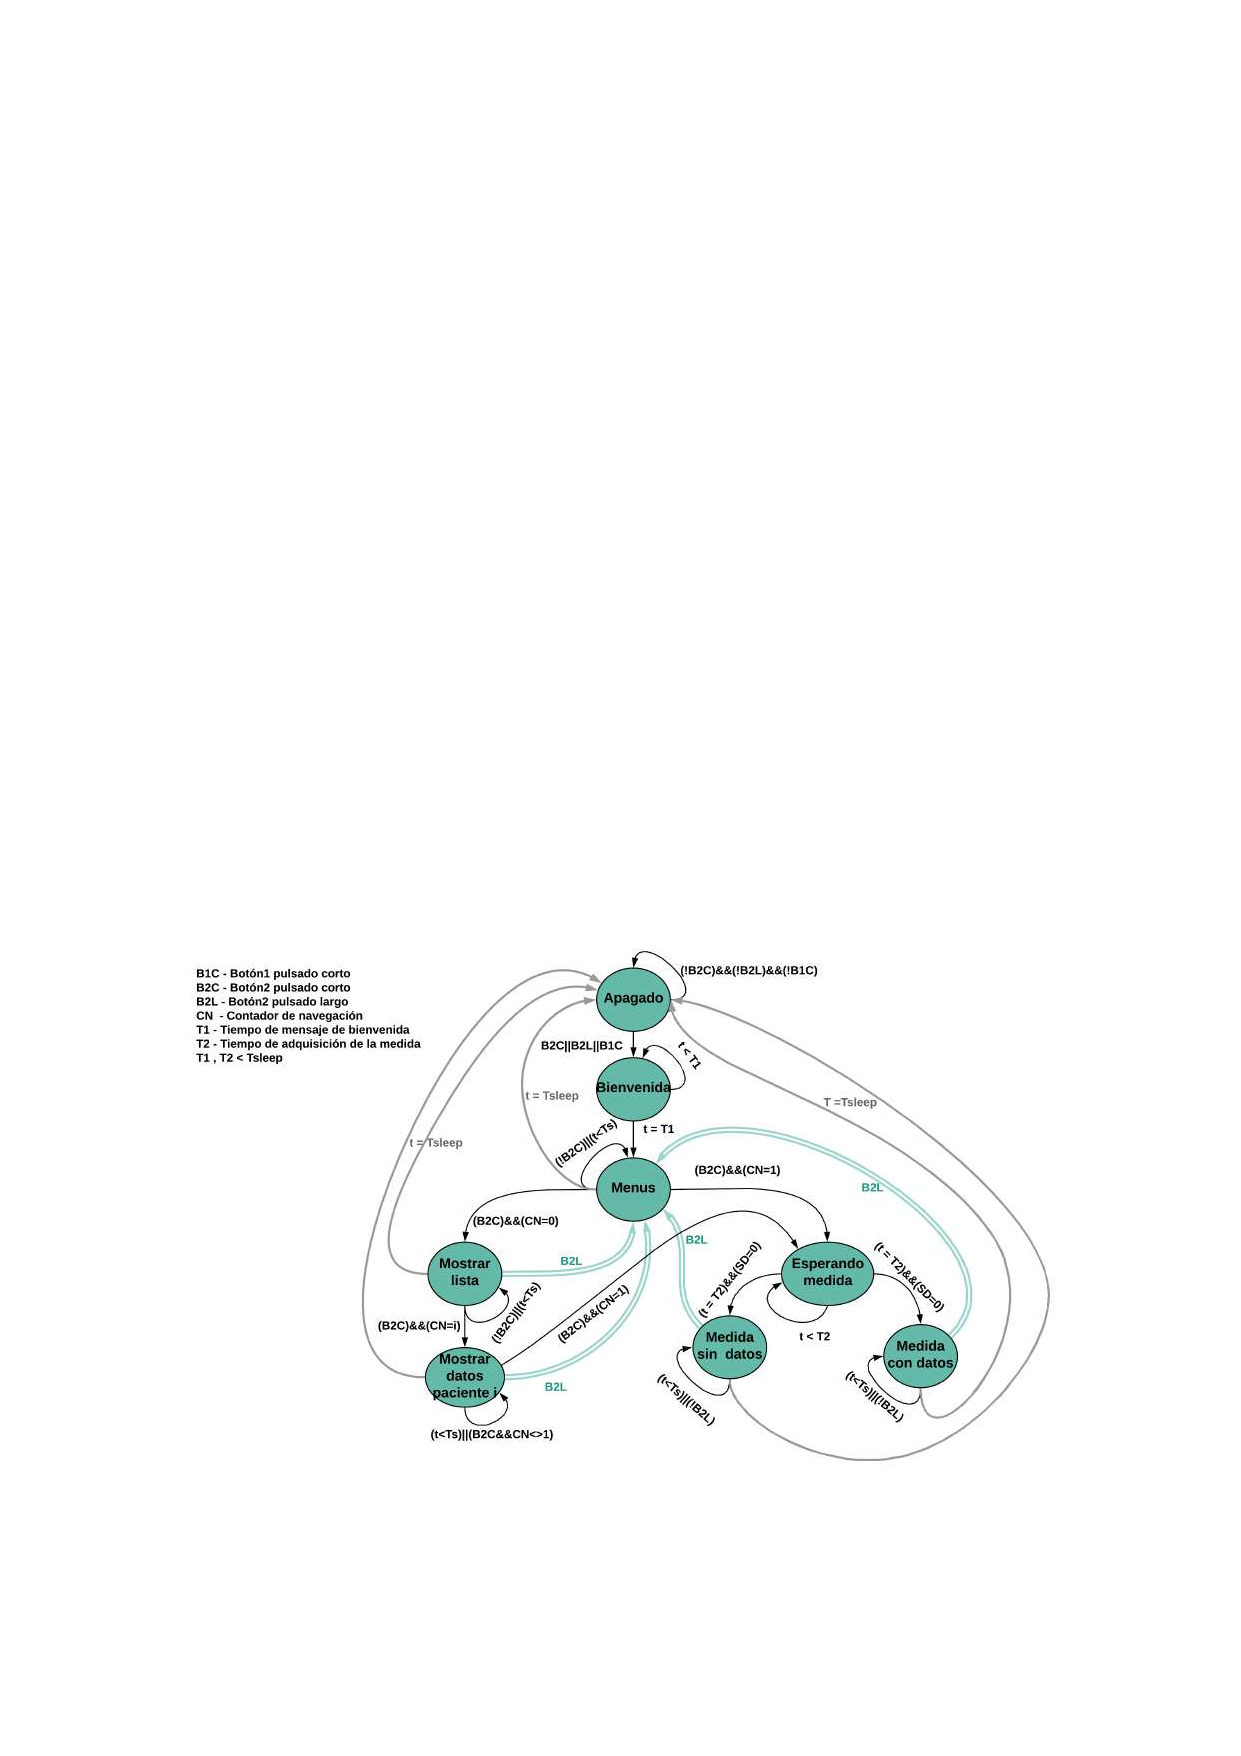
\includegraphics[width=0.9\textwidth]{maquina.pdf}
  \end{center}
  \caption{Diagrama en máquinas de estados (reproducida de \cite{cabrera2019}). }
  \label{fig:maquina}
\end{figure}
%-----------------

Explicar la elecci\'on de la arquitectura de software (Round-Robin, Round-Robin con interrupciones, encolado de funciones o RTOS). Justificar en base a tiempos de respuesta y necesidades de prioridades. Explicar qué se procesa a nivel de \textit{ISR} y \textit{main} y qué criterios se tomaron para esas elecciones.

Mencionar si se tomaron las precauciones para generar c\'odigo independiente del hardware. Mencionar qué c\'odigo representa la HAL (hardware abstraction layer). Discutir grado de portabilidad, escalabilidad y extensibilidad es decir: 

\begin{enumerate}
 \item \textit{portabilidad:} qué se debe cambiar si se cambia HW (por ejemplo microcontrolador o cambio de alg\'un periférico que tenga otro protocolo de comunicaci\'on).
 \item \textit{escalabilidad:} qué se debe agregar si a la implementaci\'on existente se desea agregar nuevas funciones (por ejemplo que acepte
 nuevos comandos, se agreguen nuevos mensajes de error).
 \item \textit{extensibilidad:} qué se debe agregar si a la implementaci\'on existente se agrega HW nuevo, por ejemplo otro sensor.
\end{enumerate}

Explicar si hay problemas de datos compartidos, qué precauciones se tomaron y mencionar qué se está haciendo para minimizar el consumo, si es que se minimiza (si no se hace nada indicarlo).


%++++++++++++++++++++++++++++++++++
\section{Pruebas y Mediciones}
\label{sec:pruebas}

Describir el setup de prueba y m\'etodos (es decir descripci\'on de las pruebas y sus resultados). 

Presentar perfil del consumo usando EnergyTrace\textsuperscript{TM}. Mostrar tiempos de ejecución de funciones, rutinas, m\'etodos o procesos (agregar diagramas de tiempos). Incluir un reporte de uso del hardware del microcontrolador (mapa de memoria, Flash, cantidad de pines utilizados, etc.).

Agregar toda otra informaci\'on relevante relacionado con pruebas y mediciones que muestren si los objetivos se cumplieron o no.

Explicar cómo se obtuvieron los resultados y qué funciones del IDE se utilizaron para ver variables, registros, memoria, etc. Si hace falta, adjuntar capturas de patallas del IDE en modo debugger mientras se hacen pruebas.

No deben faltar las explicaciones de las gr\'aficas que se adjunten, as\'i como los nombres y las unidades en los ejes de las mismas. Agregar informaci\'on en forma de tablas si se considera tambi\'en relevante (ver ejemplo en Tabla \ref{Tab:consumo}.

 \begin{table}[ht]
 	\centering
 	 		\caption{Ejemplo de Tabla. La leyenda va arriba. No hay líneas verticales. Expresar los números con igual cantidad de cifras significativas. No olvidar poner las unidades.}
 	\begin{tabular}{lccccccc}
 		\hline \hline
 		 			& Ch1	& Ch2   & Ch3   & Ch4   & Ch5   & 	   \\ \hline 
 	   A   		&			& 			  & 		  & 		  & 			 & 	  \\ \hline
 	   B        	&			& 			   & 		   & 		   & 			  &    \\ \hline
 	   C      		&			& 			  & 		  & 	 	 & 			   &    \\

 		 \hline 
 		\end{tabular}
 		\label{Tab:consumo}
\end{table}

%++++++++++++++++++++++++++++++++++
\section{Conclusiones}
\label{sec:conclusiones}

Resumir el trabajo realizado y los resultados relevantes. Mencionar qué fue lo que sali\'o mal o qué etapas del proyecto no se pudieron 
cumplir y el motivo. Discutir en relaci\'on a los objetivos, qu\'e se cumpli\'o y que no.  Analizar ventajas y desventajas de las soluciones implementadas as\'i como tambi\'en la capacidad para escalar o cambiar el hardware de base. Si corresponde y se disponen de m\'etricas para realizarlo, armar una tabla de comparaci\'on de desempe\~no  con otros sistemas similares. 


%++++++++++++++++++
\section{Anexo}
\label{sec:anexo}

\subsection{Conceptos del curso aplicados al proyecto}

Conceptos del curso aplicados al proyecto (justificaci\'on adecuada del dise\~no e implementaci\'on basados en los conceptos tratados en el curso). Este anexo debe contener un detalle de los conceptos del curso aplicados al proyecto. En el cuerpo del documento eventualmente se mencionar\'an algunas de estas consideraciones, pero el prop\'osito del presente anexo es agrupar y resumir todas las consideraciones mencionadas, y otras que por razones de extensi\'on no se incluyan en el cuerpo del documento.

\subsection{Planificaci\'on del proyecto}

Planificaci\'on del proyecto (cr\'itica, reflexiones, etc. sobre: comparaci\'on entre planificaci\'on y ejecuci\'on, horas estimadas y efectivamente dedicadas).

\subsection{Especificaci\'on del proyecto}

Incluir la especificaci\'on del proyecto (documento ya entregado, sin cambios). 

%++++++++++++++++++++++++++++++++++++
\addcontentsline{toc}{section}{Bibliograf\'ia}
\renewcommand{\refname}{Bibliograf\'ia}
\bibliographystyle{IEEEtran}
\bibliography{refs}



\end{linenumbers} %COMENTAR PARA SACAR NUMERACION DE LINEAS

\end{document}
